\documentclass[runningheads,a4paper]{llncs}
% \documentclass{article}
\usepackage{amssymb}
\usepackage{amsmath}
\setcounter{tocdepth}{3}
\usepackage{graphicx}
\usepackage{url}
\usepackage[algoruled, vlined,linesnumbered]{algorithm2e}
\usepackage{color}

%TODO Add figure a, b, c, d shit

\begin{document}

\mainmatter 

\title{Autonomous Realization of Simple Machines}
\author{Can Erdogan \and Mike Stilman}
\institute{Institute for Robotics and Intelligent Machines \\Georgia Institute of Technology}
\maketitle

\begin{abstract}

For robots to become integral parts of human daily experi- ence, they need to be able to utilize the
objects in their environment to accomplish any range of tasks. In this work, we focus particularly
on physically challenging tasks that push the limits on the robot kinodynamic constraints such as
joint limits, joint torques and etc. Previously, we demonstrated an autonomous planner that
instructs a human collab- orator where to place the available objects in the environment to form a
simple machine such as a lever-fulcrum assembly. In this work, we report results on the autonomous
realization of such a design by the humanoid robot Golem Krang, focusing on the challenges of
autonomous perception, manipulation and control.

\end{abstract}

\section{Introduction}

The ability to use the available objects in the environment towards accomplishing goals is essential
to thriving in challenging circumstances. Everyday examples of tool use include simple machines such
as levers and pulleys. The challenge in autonomous design of such simple machines is the space of
discrete choices for the component options and the related high-dimensional continuous configuration
space of the chosen components.

In previous work \cite{erdogan2013planning,erdogan2014incorporating}, we demonstrated the
constraint satisfaction approach to assembly design, specifically for robotic manipulation and
locomotion. The idea is to represent the constraints between the components of the design and on the
robot kinodynamics as generic equality and inequality functions within an
optimization framework and solve for the global minima. Operations research
\cite{vidal2006branching} and architecture \cite{yu2011make} fields also use global optimization
in design problems.

In this work, we take the next step towards full autonomy where the humanoid robot, Golem Krang,
autonomously manipulates the objects in its environment to construct a simple machine. The robot
perceives the available objects, specifically 15 kg cinder blocks and 10
kg wooden blocks (e.g. potential levers), relocates them to the desired configurations output
by the constraint planner, and actuates them to flip a 50 kg load. Figure \ref{fig:showOff} demonstrates key scenes
from this scenario such as (a) detection of a cinder block, (b) locomotion with a heavy load, (c)
manipulating a lever while subject to multiple constraints and (d) application of force to the lever
leading to a successful load motion.

\begin{figure}[ht!] 
  \centering
  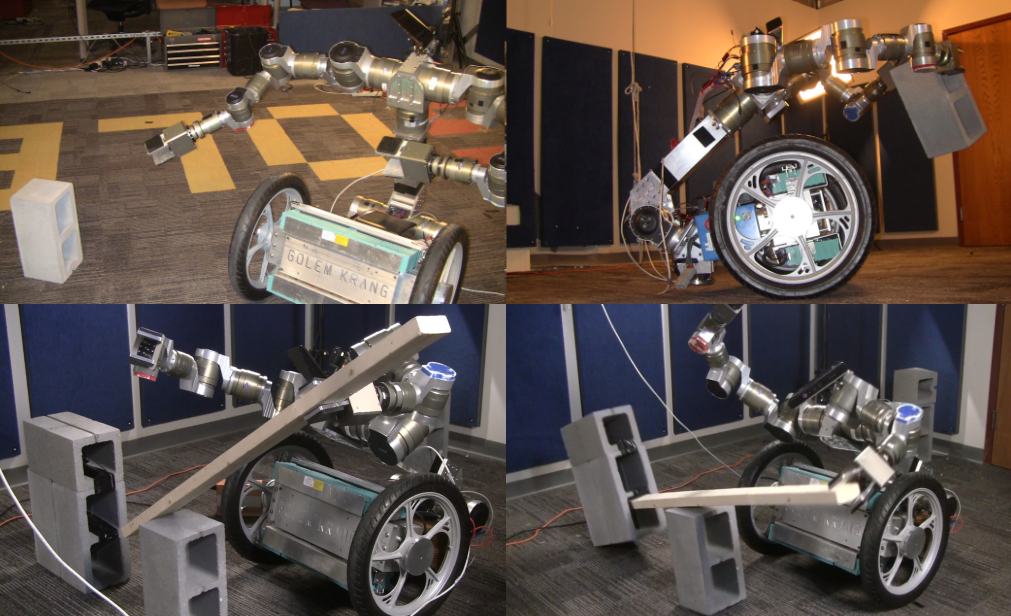
\includegraphics[width=1.0\linewidth]{Figures/showOff.png}
  \caption{The mechanical advantage in forces}
  \label{fig:showOff}
\end{figure}

Significant effort has been demonstrated by \cite{beetz2010cram,stilman2005navigation,kemp2007challenges} to incorporate autonomous agents in human environments. Our work stands
out in multiple aspects from the established state of the art. First, Golem Krang is a two-wheeled
balancing robot, similar to a segway with two 7-dof robotic arms installed. The challenge with
such a platform is the dynamic stability constraint where the robot has to ensure its center of mass
is close to the wheel axis at all times as opposed to legged or multi-wheeled platforms. Secondly, to the best of our knowledge,
Golem Krang is the tallest and heaviest two-wheeled robot with 150 kg at 1.9 m, a unique property
among similar designs \cite{kuindersma2009dexterous}. At this scale, the
weight can help with heavy-duty manipulation but also complicates the autonomous locomotion. Lastly,
Golem Krang perceives its environment with an onboard RGBD sensor with two degrees of freedom that
can be manipulated for gaze control. Autonomous perception and scene recognition has only
recently started to gather interest in the humanoid robotics field
\cite{srinivasa2010herb,nishiwaki2000design} as opposed to the established motion capture methods
\cite{dasgupta1999making}.
% 
% \section{Technical Approach}
% 
% \subsection{Constraint Satisfaction for Simple Machine Designs}
% 
% The manipulation of multiple objects to achieve a goal can be readily represented in a constraint
% satisfaction paradigm where the constraints represent the relationships between the design
% components. In this work, we focus on simple machine designs such as lever-fulcrum assemblies or
% inclined planes that need to be structurally stable and provide mechanical leverage to their users.
% Reasoning about such design criteria requires analysis of more detailed concepts such as center
% of masses, robot kinodynamic constraints and physics principles. 
% 
% The design process is composed of three steps. First, from the set of available objects
% in the environment, the planner needs to choose a subset that will be incorporated in the structure. Second,
% the structure components are assigned roles that designate how they should be put together - specifically,
% the constraints that \textit{bind} one to another. Lastly, the planner needs to configure the objects
% such that the role constraints and the general design criteria are satisfied. 
% 
% \subsubsection{Component Choices}
% 
% A completeness property for a structural design planner is a crucial advantage
% for deployment in real-world applications (e.g. military or search-and-rescue operations). In
% emergency situations, when physical challenges require creative reasoning, the ability to consider all possible solutions and determine
% if one succeeds is a critical advantage. 
% 
% The planner needs to exhaustively search the 
% entire \textit{finite} space of discrete assignments. In comparison to continuous choices, such as
% object configurations, the discrete nature of the component choices (i.e. in or out) makes such a search
% feasible. Despite the finite space, it is challenging to evaluate
% every option since there is still a combinational number of roles and infinite 
% space of configurations to reason about. Note that we assume every object is used only once in the 
% structure as opposed to the robot changing the structure throughout its use.
% 
% 
% To remedy the computational challenge, pruning strategies and heuristics are significant tools in
% cutting back the search at the top level. For instance, in construction a lever-fulcrum design,
% two wooden blocks of the same size (or approximately to a degree of confidence) can be categorized
% under one class. Similarly, for loads that are known to be heavier than the maximum load a robot can
% handle, the longer lever candidates might be prioritized in the search.
% 
% \subsubsection{Object Roles} 
% 
% Imagine that a two-step stairs is needed to enable a swarm of rough-terrain vehicles, such as 
% PackBots or RHexs \cite{yamauchi2004packbot,saranli2001rhex}, to climb a window and survey a building, and some of the vehicles have robotic
% arms that can stack box-like objects. The goal for a planner would be to choose three boxes and
% stack two of them (e.g. box B on C) such that the swarm can first climb one step and then move on to
% the two stack, until it reaches the window sill. 
% 
% In coming up with this solution, two types of choices are made. First, among the three objects,
% say A, B, and C, which object will be used as the first step and which one will be at the top
% in the second step needs to be decided. Secondly, in order to place an object on a surface, a base
% face needs to be chosen - in fact, doing so partitions the configuration space of the objects even
% before the design constraints are considered to prune infeasible assignments.
% 
% Hence, the goal of  assigning a role to an object is to specify (1) the relationship of a component with respect to
% others, and (2) which of its face and edges are used in these connections. Figure \ref{fig:matches} 
% \cite{erdogan2014incorporating} depicts some outcome assemblies with a triangle prism
% acting as fulcrum positioned on different base faces and in contact with a lever
% on various edges. We also observe that the lever can contact the fulcrum on two faces
% (discounting symmetries) that lead to feasible assemblies. 
% 
% \begin{figure}[ht!] 
%   \centering
%   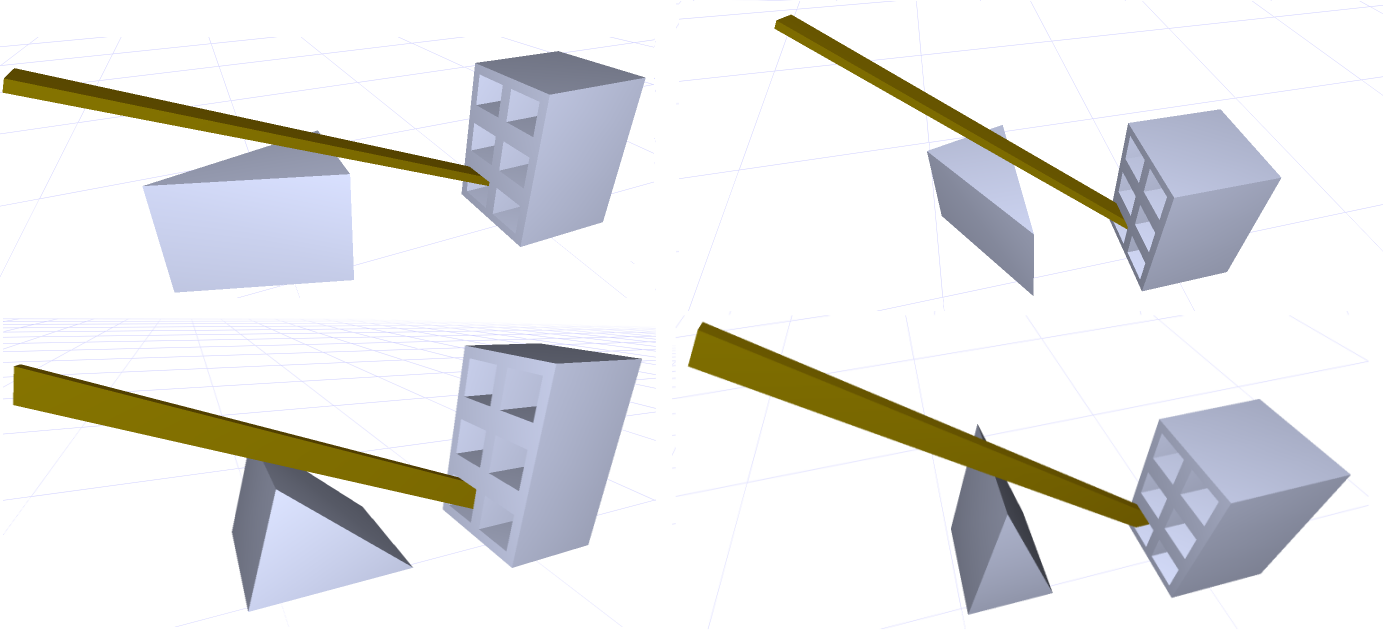
\includegraphics[width=0.7\linewidth]{Figures/matches.png}
%   \caption{Different face and edge assignments for a lever-fulcrum assembly. Some assignments,
%   such as using the shortest edge of the lever to connect the fulcrum and the load, may not
%   be feasible due to design constraints and collisions.}
%   \label{fig:matches}
% \end{figure}
% 
% Role assignment to available resources has been a thoroughly studied area, starting from
% classical planning \cite{newell1961gps,mccarthy1963programs}, and evolving into operations research
% \cite{fulkerson1961network,taha1975integer}. In this work, we adopt the STRIPS representation \cite{fikes1972strips}
% as a method to represent the domain knowledge of possible actions that can be taken on the available
% objects in the environment. For instance, a lever can be \textit{placed}
% on a fulcrum or a ramp can be \textit{rested} against another object. A minor difference in our
% framework is that every action induces additional constraints to the assembly configurations and
% an action can be taken if and only if there exists some configuration that satisfies the accumulated
% constraints.
% 
% \subsubsection{Continuous Configuration Space and Constraints}
% 
% The proposed framework accumulates design constraints via a classical planning framework
% and a feasibility process determines whether the constraints can be satisfied by some configuration
% of the components. Different types of constraints can all be generically
% expressed as equality or inequality functions on the space of object and robot configurations.
% If all the constraints are convex, for instance in a stair or bridge design with simplified
% robot assumptions, the feasibility can be determined by an efficient simplex algorithm
% implementation \cite{erdogan2013planning}. For nonconvex domains, especially when
% robot kinodynamics are considered, we propose a nonlinear optimization process which minimizes the
% violation of the constraints and attempts to find an assignment of configurations that satisfies all of them.
% 
% A number of design constraints such as stacking a box on top of another one or placing a lever
% at the edge of a fulcrum can be expressed with geometric projections. Figure \ref{fig:constraints}
% demonstrates three types of connections: (1) center of mass-face, (2) edge-face, and (3) face-face. 
% The general idea is that points of interest such as center of mass, endpoints of an edge or vertices
% of a face are projected to the plane of another face and limits are imposed on its location. For instance,
% for two objects to be stacked successfully (A), the center of mass of the top object has to lie within
% the supporting face of the bottom object. Similarly, to ensure an edge is on a face (B), it is sufficient
% to confine the endpoints of the edge onto the face plane and guarantee there exists a shared point
% (e.g. cross) between the edge and the face. Lastly, for contact between two faces (C), 
% three points of one of the faces has to lie on the other one and again, a shared point should exist.
% Observe that geometric contact concepts are easily expressed through equality
% and inequality expressions on the projections of significant points on the meshes. 
% 
% \begin{figure}[ht!] 
%   \centering
%   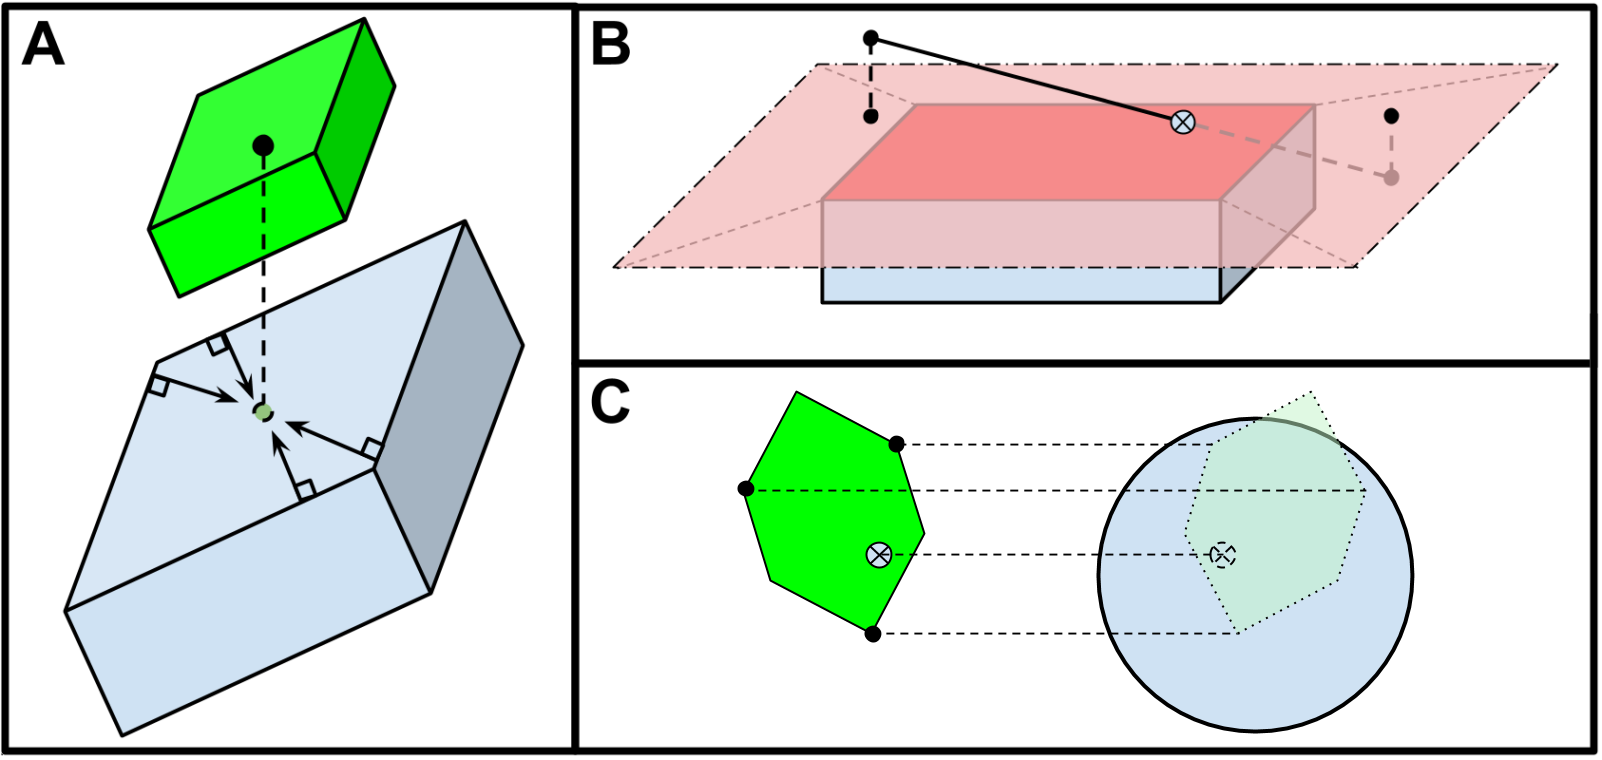
\includegraphics[width=0.75\linewidth]{Figures/constraints.png}
%   \caption{Visualization of different types of geometric contact constraints}
%   \label{fig:constraints}
% \end{figure}
% 
% Once the object choices and roles are determined, the equality and the inequality constraints between
% the assembly components can be gathered into two sets $\mathcal{F}$ and $\mathcal{G}$ respectively.
% The idea behind using optimization to find feasible samples in the configuration space is based on
% creating error functions by the violation of the constraints for a sample design $\vec{x}$:
% 
% \vspace{-1em}
% \begin{align*}
% f(\vec{x}) = 0 \;\; \Rightarrow & \;\; E_f(\vec{x}) = f^2(\vec{x}) \\
% g(\vec{x}) \leq 0 \;\; \Rightarrow & \;\; E_g(\vec{x}) = 
% 	\begin{cases}
% 		g^2(\vec{x}) & \text{if $g(\vec{x}) > 0 $}, \\
% 	0        & \text{otherwise}.
% 	\end{cases}
% \end{align*}
% 
% \noindent where $E_f(\vec{x})$ and $E_g(\vec{x})$ are the proposed squared error functions. Now,
% given the constraint sets $\mathcal{F}$ and $\mathcal{G}$, we define the total error:
% 
% \begin{equation}
% 	\mathcal{E}(\vec{x}) = \sum\limits_{f \in \mathcal{F}} E_f(\vec{x}) + \sum\limits_{g \in \mathcal{G}} E_g(\vec{x}).
% \end{equation}
% 
% \noindent Note that $\mathcal{E}(\vec{x})$ is 0 for
% some $\vec{x}$ if and only if configurations $\vec{x}$ satisfy all the design
% constraints. Moreover, the global minima is guaranteed be more than or equal
% to 0 since the function is a sum of squared errors. Then, by using an optimization method, such as
% Levenberg-Marquardt, the global minima can be found through sampling the space for good initializations.
% 
% We outline the overall approach in Algorithm 1 below. Given the available objects, the goal
% criteria and the available actions, the planner searches in the space of discrete object roles
% (line 3) and attempts to take actions as long as they lead to feasible configurations (line 9). The forward
% search accumulates constraints until a feasible design is reached or backtracks. 
% 
% %TODO Comment the algorithm
% \begin{algorithm}[ht!]
%   \SetCommentSty{emph}
%   \KwIn{$domain$: objects properties and generic actions; $goals$: list of goal literals to be fulfilled; $initialState$: discrete literals and no constraints; }
%   \KwResult{configurations: a feasible value in goal subspace; }
%   $stateStack \leftarrow $createStack$(initialState);$ \\
%   \While{$state \leftarrow stateStack$.pop$()$} {
%     $actions \leftarrow $stateActions$(domain)$; \\
%     \ForEach{$action$ in the set $actions$} {
%       \If{$action.pres \subset state.literals$} {
% 				newConsts $\leftarrow$ state.consts $\cup$ action.consts; \\
% 				\For{$counter = 1 \dots MAX\_COUNT$} {
% 					\{\textit{localMin, confs}\} $\leftarrow $optimize($newConsts$, newSeed($domain$)); \\
% 					\If{abs$(localMin) \leq 1e^{-4}$} {
% 						\lIf{$goals \subset action.afters$} \Return{confs}; \\
% 						\Else{
% 							$child = \{state.literals \cup action.afters, newConsts\}$ \\
% 							$stateStack$.push($child$); \\
% 							\textbf{break}; \\
% 						}
% 					}
% 				}
% 			}
% 		}
%   }
%   \Return{$\emptyset$}; 
%   \caption{ConstraintPlanner()}
% \end{algorithm}
% 
% \subsection{Humanoid Robot Platform: Golem Krang}
% 
% Designed and built in the Humanoid Robotics Laboratory, Golem Krang is a 150 kg, 6.2 m segway-like
% humanoid robot with two wheels that uses a balancing strategy for locomotion and manipulation
% \cite{stilman2010golem}. Given its unique design, the proposed planner needs to address several
% constraints. First, the contact point on the lever needs to be reachable by the robot.
% Second, the robot needs to apply sufficient force to overcome the opposing weight or friction, but
% we still need to maintain a maximum force limit to protect the motors. Lastly, Golem Krang needs to
% maintain a stable posture before contact is made with the structure.
% 
% \subsection{Perception}
% 
% Equipped with a Microsoft Kinect that can pan and tilt, Golem Krang can inspect and reason about its
% environment with visual data. In perceiving the environment, we propose using a light-weight
% feasure-based recognition approach as opposed to full 3D based approaches that use the entire mesh
% data such as the iterative closest point algorithm or over-segmentation methods. 
% An assumption is that the planner knows the meshes of the available objects and with minimal
% additional feature knowledge, such as the top of a cinder block is at 44 cm from the ground or a
% lever is at least 2 meters in one dimension, we can speed up the detection. The proposed approach,
% detects individual and/or assembly of cinder blocks, walls and wooden blocks
% as shown in Figure \ref{fig:detection}. 
% 
% \begin{figure}[ht!] 
%   \centering
%   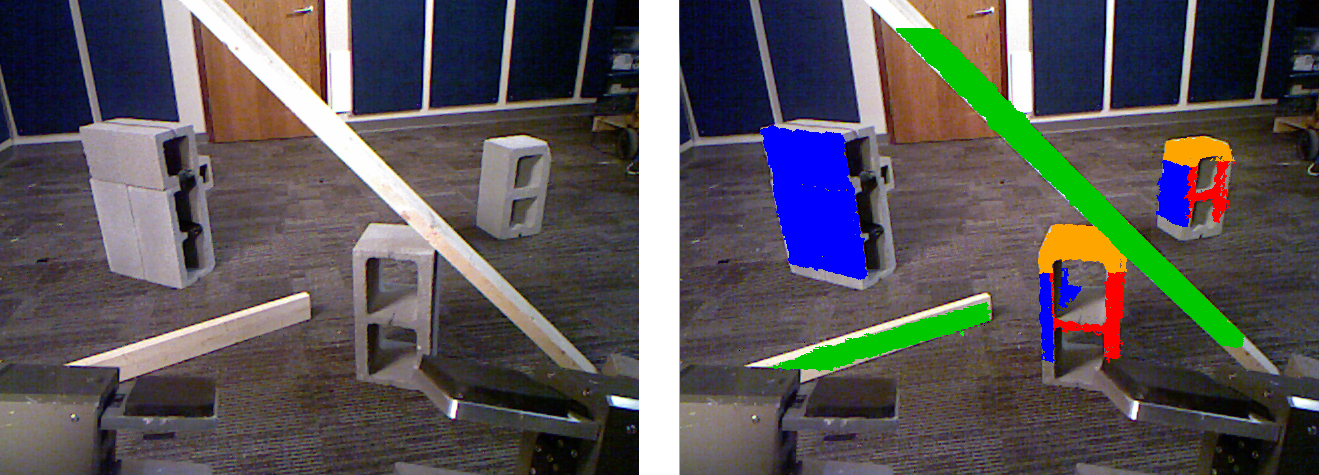
\includegraphics[width=0.9\linewidth]{Figures/detection.png}
%   \caption{Cinder block and wooden plates detected as fulcrum and lever objects.}
%   \label{fig:detection}
% \end{figure}
% 
% 
% \subsection{Locomotion}
% 
% The primary locomotion strategy for Golem Krang is to balance on its two wheels, keeping its
% center of mass on the vertical plane through its wheel axis. Modeled as an inverted pendulum,
% locomotion via balancing has a few advantages over running on both the wheels and the back caster.
% First, the footprint of the robot is smaller, 54 cm in width due to the wheel diameter
% while balancing, as opposed to 86 cm when the robot is grounded. Second, the
% locomotion is simpler to model since the fixed caster without omnidirectional wheels
% sustains different ground reaction forces as the robot spins, moves forward and backward. 
% 
% The position and posture control is implemented using a proportional derivative controller based on
% the inertial readings that indicate the robot angle from the vertical and the wheel encoders. In
% this work, we assume the environment is setup such that the locomotion can be carried out by
% turning towards the goal position, moving forward and adjusting for the goal orientation - ignoring
% collisions in the world. To move forward, we use a velocity profile with limits on minimum and maximum
% acceleration and deceleration. A significant aspect of the locomotion is the manipulation of heavy
% objects such as 15 kg cinder blocks and 10 kg wooden plates. To enable stable dynamic balancing, the
% force-torque sensors at the grippers are used to incorporate the mass of the
% carried objects in the computation of the center of mass position. 
% 
% \subsection{Manipulation}
% 
% The manipulation of multiple objects under motor and perception uncertainty requires a series of 
% robust strategies both algorithmically and in practical implementation. In this work, a wide range of
% motion planning tools are adopted such as rapidly-expanding random trees (RRTs) \cite{kuffner2000rrt},
% analytical inverse kinematics \cite{tolani2000real} and Jacobian control \cite{whitney1969resolved}. 
% Additionally, we propose using guarded moves \cite{bejczy1977effect} 
% that control the manipulator behavior until a predetermined tactile feedback is received. Moreover,
% ``conformant motions'' are used where the robot forces itself
% and its environment to a desired state without sensory feedback \cite{goldman1996expressive}. 
% % 
% \subsubsection{Motion planning}
% 
% Figure \ref{fig:manipulation} depicts the analytical inverse kinematics and the 
% steps during the manipulation of a cinder block to be used as a fulcrum. We use a predetermined
% grasp location, the top surface with the holes at the sides (see Figure \ref{fig:manipulation}a).
% The planner first uses analytical
% inverse kinematics to find configurations close to the object that are collision-free.
% Figure \ref{fig:manipulation}a displays three configurations out of which the left most,
% semi-transparent one collides with a wheel. Once a goal in arm jointspace is determined,
% bidirectional RRTs with path shortening and smoothing are used to move the arm from its initial 
% pose to the goal. Figure \ref{fig:manipulation}b demonstrates the keyframes as the arm moves
% from its initial pose (red), around the cinder block to avoid collisions, until it reaches the goal
% pose (green) in front of the grasp point. 
% 
% \begin{figure}[ht!] 
%   \centering
%   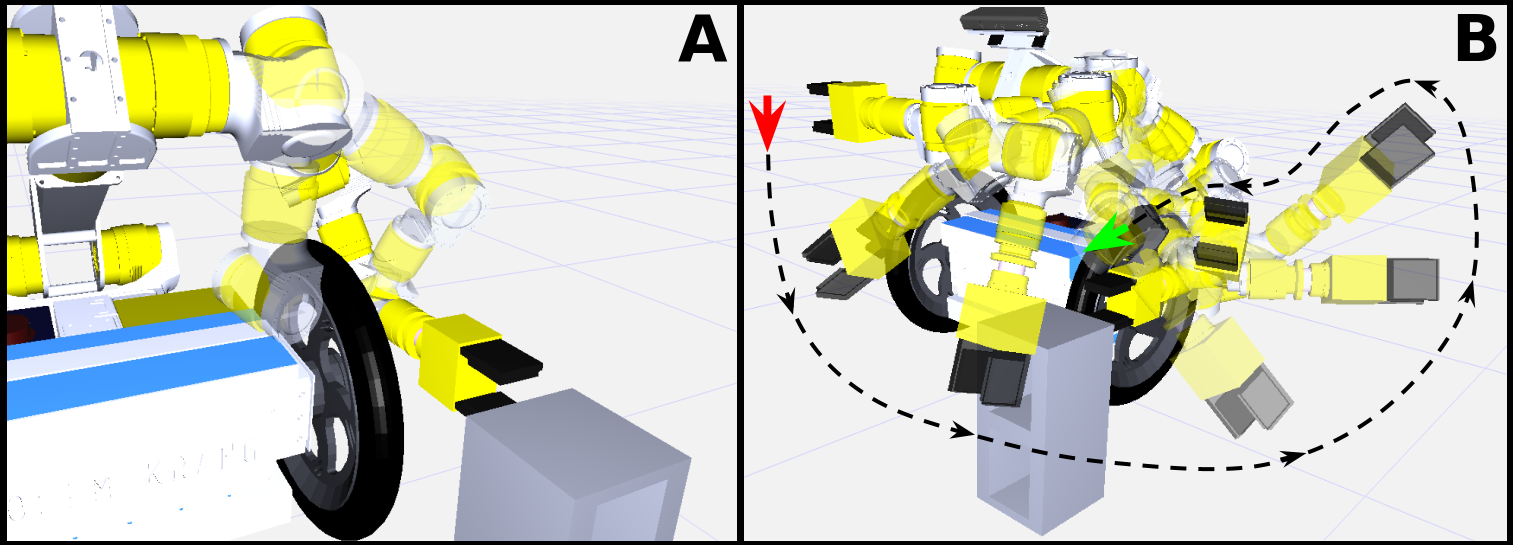
\includegraphics[width=1.0\linewidth]{Figures/manipulation.png}
%   \caption{Left: Candidate grasp poses for the block - left most in collision with wheel.
%   Right: RRT trajectory to goal grasp pose, moving around the block to avoid collisions.}
%   \label{fig:manipulation}
% \end{figure}
% 
% \subsubsection{Guarded and conformant motions}
% 
% Once in position for grasping, Golem Krang uses force/torque feedback at the end-effectors
% to reach out to the cinder block until contact and ensures its grippers can grasp it. Such guarded
% moves have proven to be simple, heuristic alternatives to visual servoing as the robot picks up
% levers and positions them on the fulcrum and inside the load.
% 
% In addition to guarded moves with sensory feedback, we also utilize conformant motions where,
% to localize the lever more precisely, the robot runs its wheels against the lever.
% When one of the wheels hit the obstacle first, the other wheel comes around until both wheels
% are in contact and any visual position error is removed.
% Such motions are used to eliminate uncertainty in the initial pose of 
% objects in assembly tasks by pushing the objects into known poses \cite{mason1986mechanics}.
% 
\section{Experiments}

Golem Krang is tasked with overturning a 50 kg load using a lever-fulcrum assembly with a limit of
300 Nm on the force it can apply to the environment. Given the dimensions of the 
available objects in the environment, the robot has to design a structure, locate the components,
configure them into their positions and actuate the simple machine. In the following section, we
describe a typical run, focusing on details of perception, locomotion and manipulation.

Placed in a random configuration in the room, Golem Krang begins by scanning the room for the 
available objects and finds the closest cinder block that would be used as a fulcrum (see Figure \ref{fig:typical_a}).
The scanning process is composed of a set of atomic behaviors which move its arms out of its sight to avoid occlusions.
Once the fulcrum is located, the robot approaches until it 
positions itself in a predetermined distance to grasp the object. Using the motion planning tools,
such as RRTs and guarded moves, the robot grasps the cinder block at its top.
%TODO Visualize the planner output

\begin{figure}[ht!] 
  \centering
  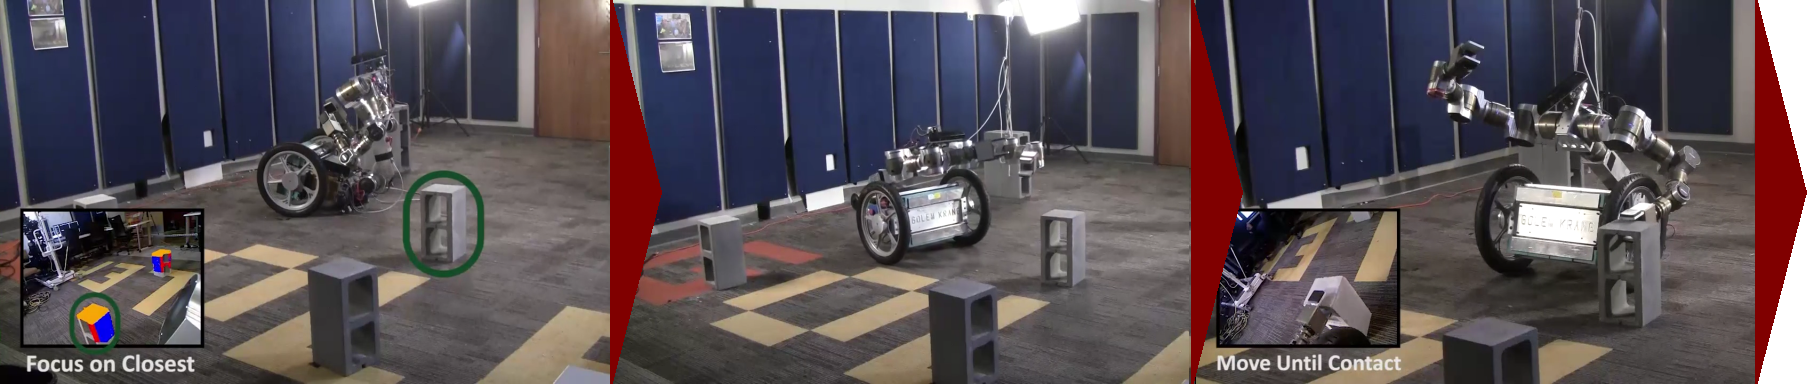
\includegraphics[width=1.0\linewidth]{Figures/a.png}
  \caption{Once Golem Krang detects the closest cinder block (left), it approaches (middle) and grasps
  the objects (right). Scene continues in Figure \ref{fig:typical_b}.}
  \label{fig:typical_a}
\end{figure}

An interesting observation we expand on in Section 4 is about how the location of a manipulated object
and the uneven distribution of its weight over the wheels affect the locomotion accuracy. To minimize
such an artifact, in Figure \ref{fig:typical_b}, Golem Krang first moves the grasped cinder block 
to the middle of its torso before turning around and localizing the load object at 50 kg. Having
detected the load, the final configuration of the fulcrum is deduced from the assembly design and
the robot places it appropriately. 

\begin{figure}[ht!] 
  \centering
  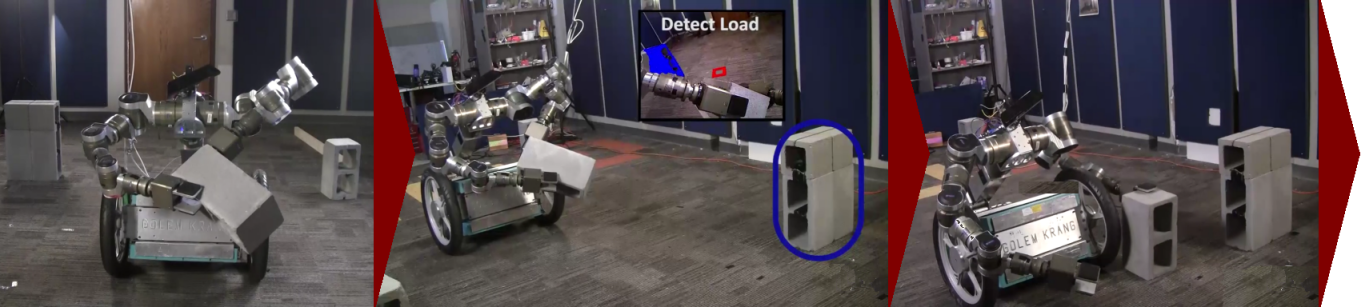
\includegraphics[width=1.0\linewidth]{Figures/b.png}
  \caption{Having grasped the fulcrum, the robot localizes the load and places the fulcrum
		in the initial design configuration. Scene continues in Figure \ref{fig:typical_c}.} 
	\label{fig:typical_b}
\end{figure}

In the third part of the experiment, Golem Krang needs to detect and localize a candidate lever
object and grasp it, as shown in Figure \ref{fig:typical_c}. Given the size of the lever and the
noisy perception data, we propose using the wheels to localize the lever object more accurately
once the robot approaches it. Figure \ref{fig:typical_c}b displays the conformant behavior where the 
robot moves forward slowly to collide with the lever and have its localization error fixed. The
left wheel first makes contact and the contact overcomes the input torque, while the right wheel 
keeps moving until the robot is parallel and directly in front of the lever. 

\begin{figure}[ht!]  	
  \centering
  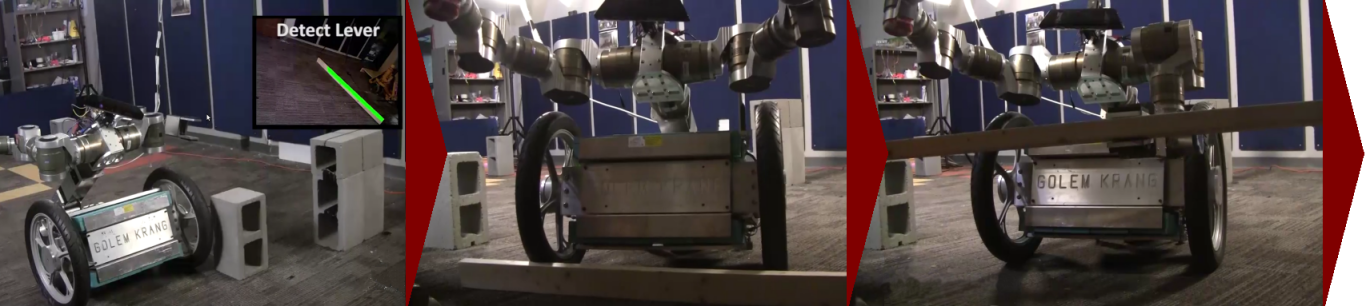
\includegraphics[width=1.0\linewidth]{Figures/c.png}
  \caption{The lever is picked up by first using vision and then running
	the wheels against the object to make physical contact before manipulation. Scene continues 
	in Figure \ref{fig:typical_d}.}
  \label{fig:typical_c}
\end{figure}

To simplify the locomotion, we have assumed collision-free paths and when Golem Krang carries the
lever, we ensure that the lever is carried high enough that it does not collide with other objects
(see Figure \ref{fig:typical_d}. Once the robot repositions itself in front of the robot, using
guarded moves, the robot first pushes the lever against the load horizontal to ensure it is at
the correct horizontal distance and then raises it until the design specification. Once at the
correct height, the robot releases the lever and allows it to slide on the fulcrum into the load
 - one of the more practically challenging tasks. For addition tasks, we have used task-constraint
 manipulation with online perception to minimize the errors during this routine. Finally, in
 Figure \ref{fig:typical_d}c, the robot pushes the object at the desired contact point and overturns
it.

\begin{figure}[ht!] 
  \centering
  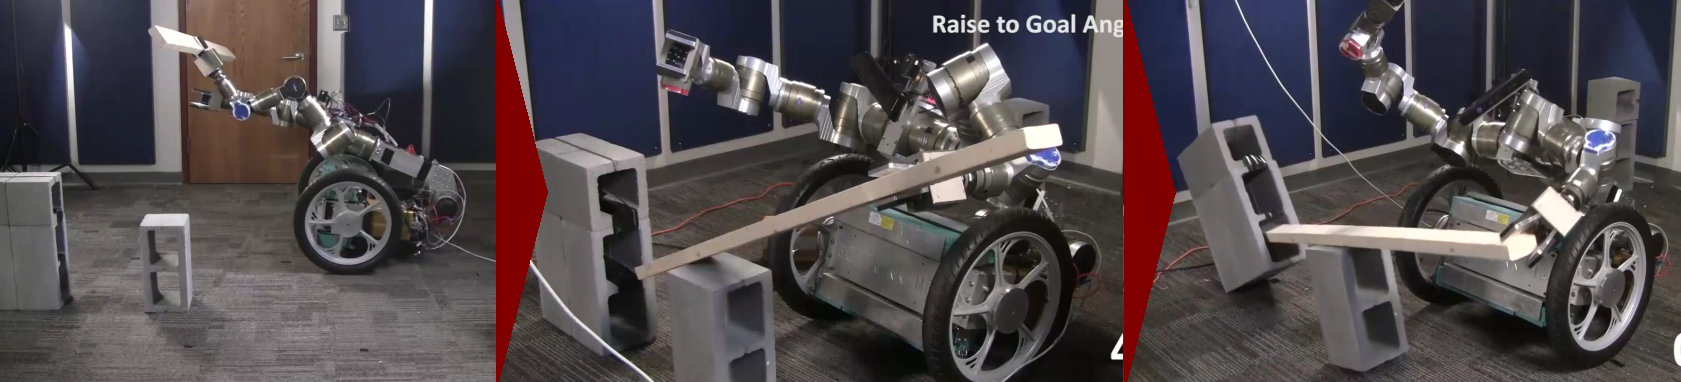
\includegraphics[width=1.0\linewidth]{Figures/d.png}
  \caption{Golem Krang places the lever in the planned pose and overturns the 50 kg load.}
  \label{fig:typical_d}
\end{figure}

% \section{Results}
% 
% In this section, we provide experimental results on the functionality of the realized simple
% machines under different conditions, study the sources of inaccuracies in the assembly process
% and provide some insights on the autonomous manipulation of heavy objects. 
% 
% \subsubsection{Designs with Different Load Weights}
% 
% The proposed framework is tested with two 
% load sizes, 50 kg and 100 kg, where the planner chooses from two levers 1.7 and 2.5
% m long. Once the design is made, Golem Krang autonomously constructs it, as
% described in Section 3, and we measure the force/torque sensor readings at the actuating arm gripper. Figure \ref{fig:graphs}a demonstrates the maximum applied forces at 242.27 Nm and 368.63 Nm for 50 kg and 100 kg experiments
% respectively. We conclude that the mechanical advantage is 2.02:1 and 2.66:1 for each case, and 
% the maximum force limit is preserved; and thus, the planned design, its assembly and actuation are
% successful.
% 
% \begin{figure}[ht!] 
%   \centering
%   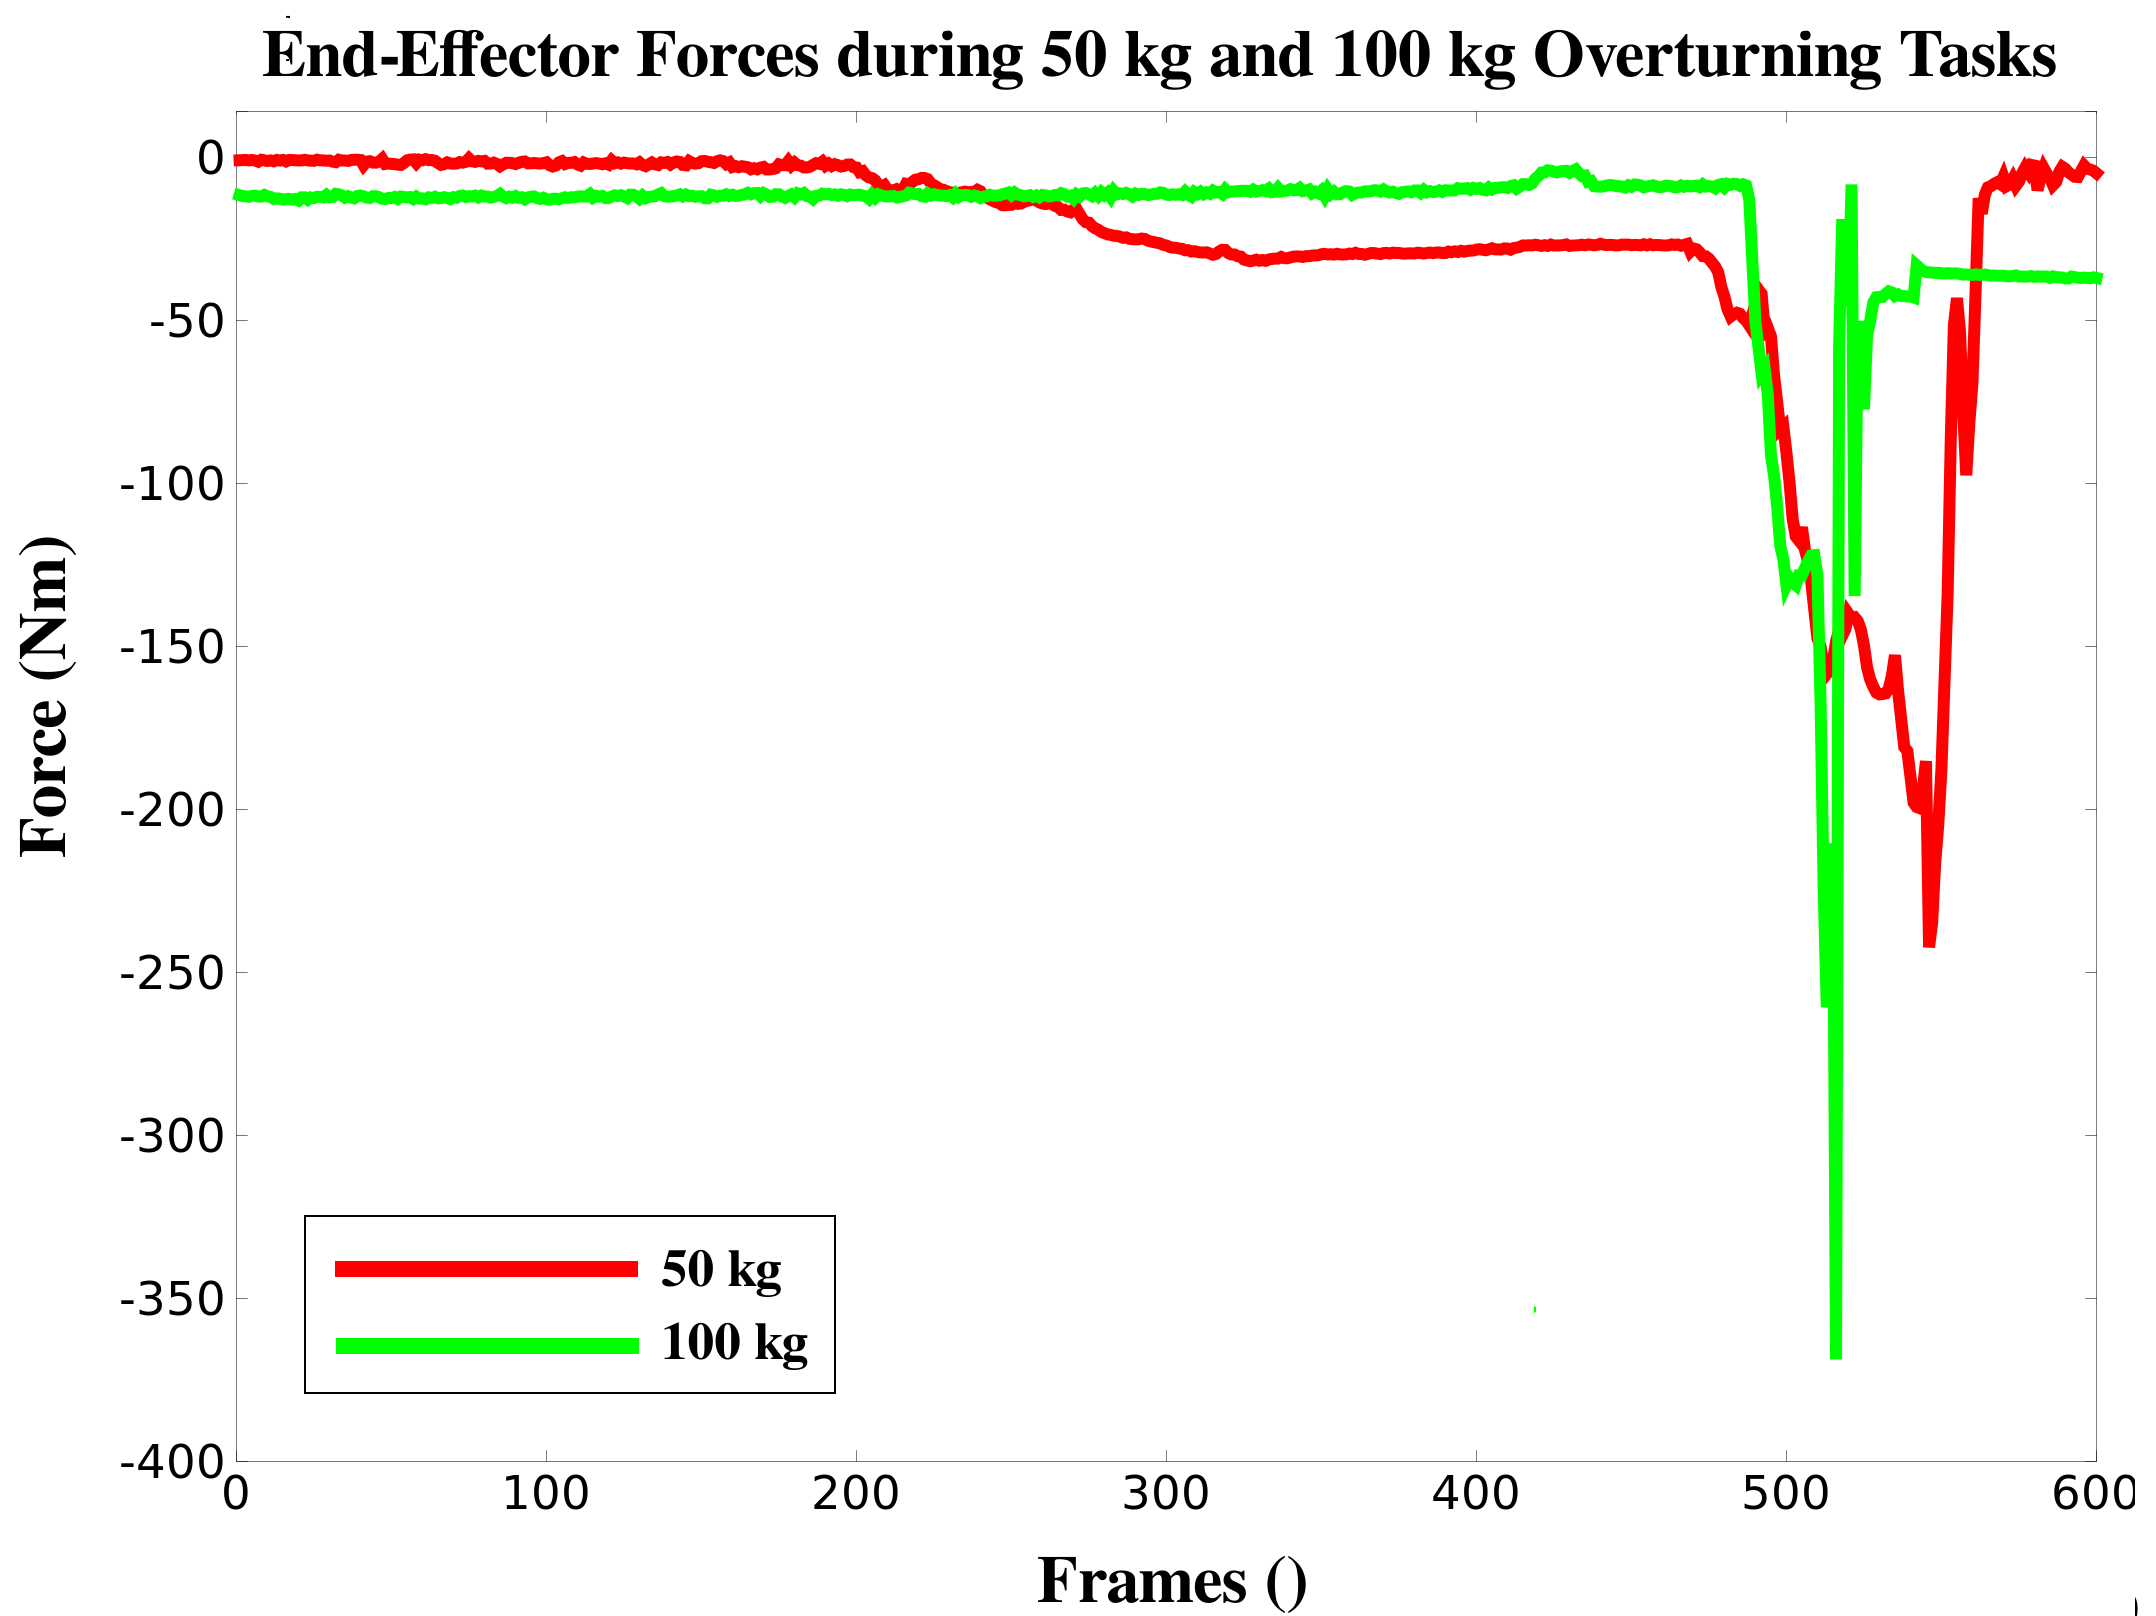
\includegraphics[width=1.0\linewidth]{Figures/loads.png}
%   \caption{Left: Input forces during the 50 kg (red) and 100 kg (red) overturning tasks. 
%   Right: Fulcrum shift while using a small lever leads to increased input force  (grey line).}
%   
%   \label{fig:graphs}
% \end{figure}
% 
% \vspace{-2em}
% \subsubsection{Fulcrum Base Choice and Unmodeled Implications}
% 
% The proposed planner focuses on the initial moment of force application and ensures that the force
% induces enough torque to overturn the load. Although constraints are used to guarantee that the
% motion is collision-free, the possibility of the the contact between
% the lever and the cinder block moving is not considered. Figure \ref{fig:short}a demonstrates a case where
% the planner \textit{autonomously} adapts the fulcrum base choice to accommodate the short
% lever. However, the fulcrum point moves (Figures \ref{fig:short}b-c) because the contact height is
% shorter than the center of mass of the load. Figure \ref{fig:graphs}b displays the increase in
% the required force as the fulcrum shifts.
% 
% 
% \begin{figure}[ht!] 
%   \centering
%   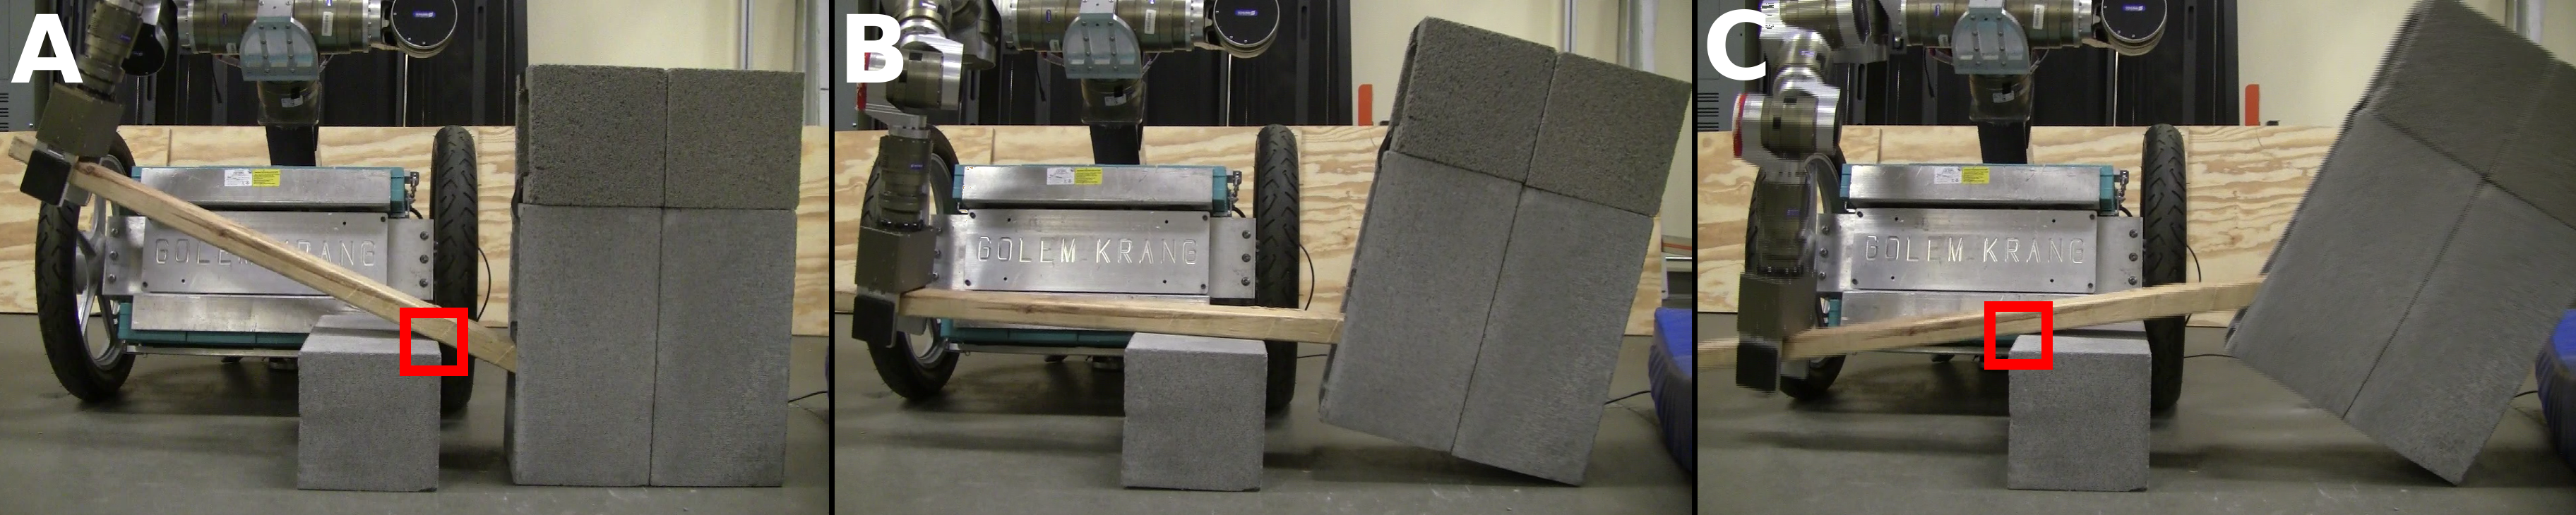
\includegraphics[width=1.0\linewidth]{Figures/short.png}
%   \caption{The movement of the fulcrum-lever contact point for short lever objects.}
%   \label{fig:short}
% \end{figure}
% 
% \subsubsection{Evaluating Accuracy}
% 
% A challenge in long-term manipulation tasks is the accumulation of error over the course of the
% executions. To remedy such an error build-up, at the current state of our work, the authors
% intervene and instruct the robot to minimize its error if necessary. One of the main causes of this
% inaccuracy is the reliability of the RGBD data. We observe that a mean error of 2-3 cm within a 1 m
% bound increases up to 10 cm with 4 meters. The proportional increase in error with respect to
% distance suggest a camera calibration problem which can be addressed with bundle adjustment \cite{pradeep2014calibrating}. 
%  
% Secondly, locomotion for heavy balancing robots is an active research area and our implementation
% with a proportional-derivative controller can be improved following techniques as presented in
% \cite{ha1996trajectory}. A major challenge is the system modeling, specifically accurate center of
% mass and inertia information. Figure \ref{fig:controller} demonstrates the behavior of the robot as
% it follows a velocity profile, moving straight. The sinusoidal behavior in the output position
% trajectory (red) is the robot regaining its balance and the steady state error may be accommodated
% with an integral term in the controller. A concern is the high-frequency velocity sinusoids which may cause instability when heavy objects are manipulated.
% 
% \begin{figure}[ht!] 
%   \centering
%   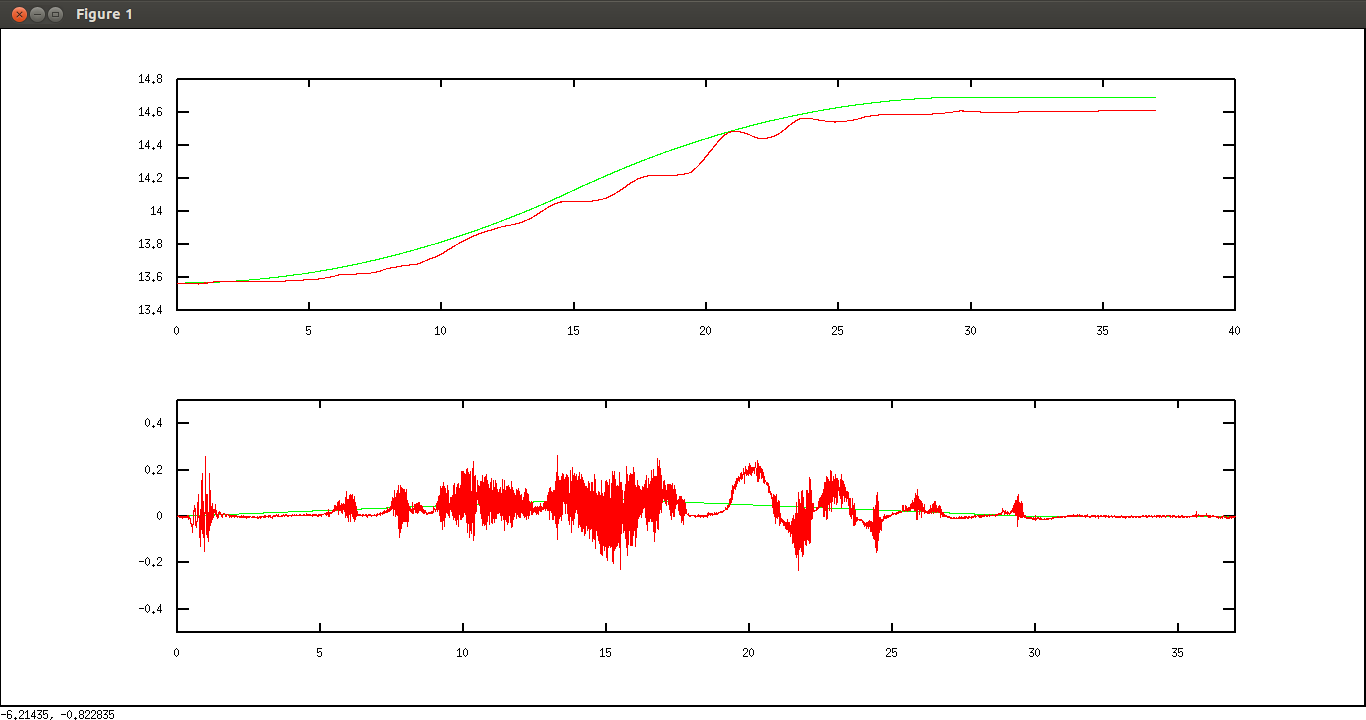
\includegraphics[width=0.9\linewidth]{Figures/controller.png}
%   \caption{The oscillations and steady state error in following a reference velocity profile.}
%   \label{fig:controller}
% \end{figure}
% 
% \subsubsection{Manipulation of Heavy Objects}
% 
% The manipulation of heavy objects brings about interesting challenging in manipulation, locomotion
% and control fields. First of all, even though the mass and the center of mass information of a
% carried load is sufficient in maintaining quasi-static balance, the inertias are needed when
% the motion become faster. Although most of the time, the dynamic parameters of manipulated objects
% is not readily available, there are a variety of methods to estimate them with simple experiments
% \cite{saal2010active} or with simplifying assumptions based on geometry and mass. 
% 
% Secondly, we observe that the configuration of the grasped object with respect to the body frame
% can affect the accuracy of locomotion. For instance, carrying a 15 kg load in the middle of the 
% two wheels as opposed to a meter off to the side induces different output trajectories for the 
% same velocity profiles. Figure \ref{fig:wheels} demonstrates the effect of the distribution 
% of the load mass over the wheels where the robot moves a cinder block from +1 meter to the -1 meter off
% its center and attempts to follow a straight line. The results show a proportional relationship
% where the trajectories bias towards the load increases with the distance between the load and the center. 
% We speculate that the cause is that the wheel with the more weight on has to apply more torque
% to keep up with the other one. Note that the distribution of the load and its effect of the joint
% torques is a general issue that also affects legged humanoid robots. 
% 
% \begin{figure}[ht!] 
%   \centering
%   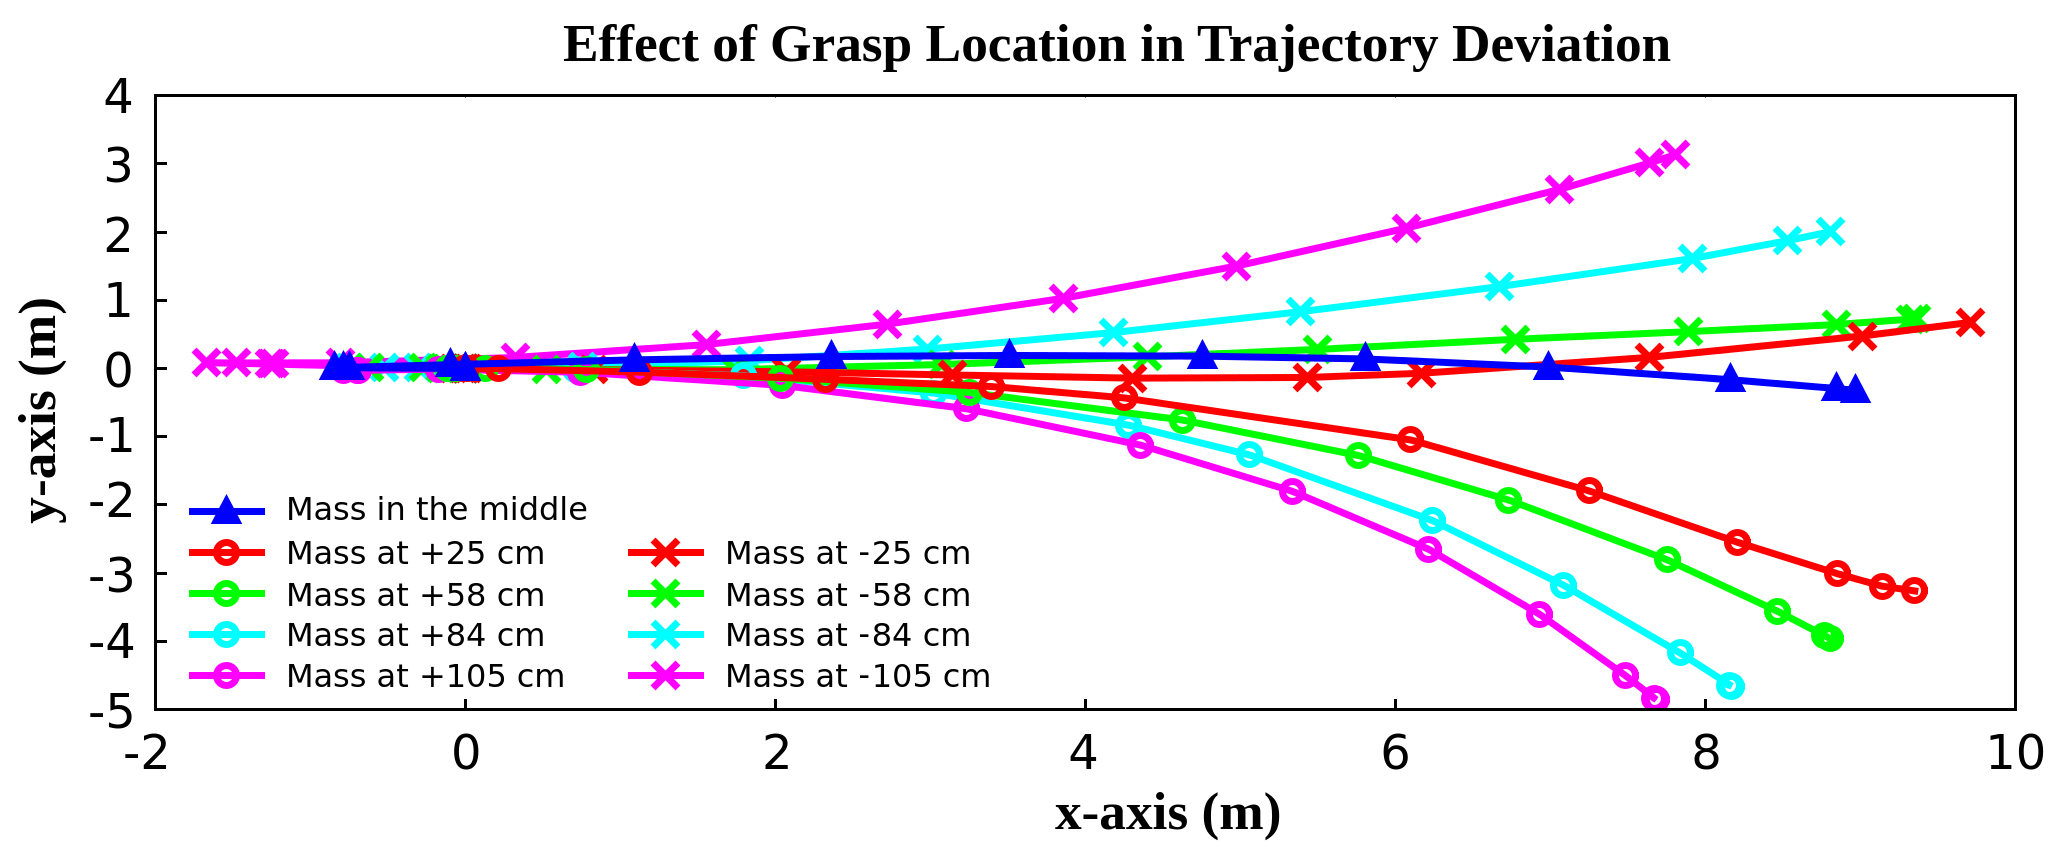
\includegraphics[width=0.9\linewidth]{Figures/wheels.png}
%   \caption{The effect of the grasping location on the accuracy of locomotion.}
%   \label{fig:wheels}
% \end{figure}
% 
% Lastly, the mass and the sheer size of the manipulated objects can cause problems with robust
% grasping during locomotion. For instance, for Golem Krang's grippers with two prismatic finger joints,
% it is important to guarantee that an object would not slip from its grasp as the robot turns around
% swiftly. To handle such cases, we have adopted a two-hand grasp for the cinder block and ensured
% that the lever is held mostly from its middle region and at an upwards angle. 
% 
% \section{Discussion}
% swiftly. To handle such cases, we have adopted a two-hand grasp for the cinder block and ensured
% swiftly. To handle such cases, we have adopted a two-hand grasp for the cinder block and ensured
% swiftly. To handle such cases, we have adopted a two-hand grasp for the cinder block and ensured
% swiftly. To handle such cases, we have adopted a two-hand grasp for the cinder block and ensured
% swiftly. To handle such cases, we have adopted a two-hand grasp for the cinder block and ensured
% swiftly. To handle such cases, we have adopted a two-hand grasp for the cinder block and ensured
% swiftly. To handle such cases, we have adopted a two-hand grasp for the cinder block and ensured
% swiftly. To handle such cases, we have adopted a two-hand grasp for the cinder block and ensured

\begin{thebibliography}{27}

\bibitem{erdogan2013planning} Erdogan, C., Stilman, M: Planning in constraint space: Automated design of
functional structures. ICRA, 2013.
\bibitem{erdogan2014incorporating} Erdogan, C., Stilman, M: Incorporating kinodynamic constraints in automated
design of simple machines. IROS, 2014.
\bibitem{vidal2006branching} Vincent, V., Geffner, H.: Branching and pruning: An optimal temporal pocl planner
based on constraint programming. AI, 2006.
\bibitem{yu2011make} Yu, L. F., Yeung, S. K., Tang, C. K., Terzopoulos, D., Chan, T. F., Osher, S: Make it home:
automatic optim. of furniture arrangement. In Siggraph, 2011.
\bibitem{beetz2010cram} Beetz, M., Mosenlechner, L., Tenorth, M: Crama cognitive robot
abstract machine for everyday manipulation in human environments. In IROS,
2010.
\bibitem{stilman2005navigation} Stilman, M., Kuffner, J. J.: Navigation among movable obstacles: Real-
time reasoning in complex environments. IJHR, 2005.
\bibitem{kemp2007challenges} Kemp, C. C., Edsinger, A., Torres-Jara, E: Challenges for robot
manipulation in human environments. IEEE Robotics and Automation Magazine,
14(1):20, 2007.
\bibitem{kuindersma2009dexterous} Kuindersma, S. R., Hannigan, E., Ruiken, D., and Grupen, R. A:
Dexterous mobility with the ubot-5 mobile manipulator. ICAR, 2009.
\bibitem{srinivasa2010herb}  Srinivasa, S. S., Ferguson, D., Helfrich, C. J., Berenson, D., 
Collet, A., Diankov, R., Gallagher, R., Hollinger, G., Kuffner, J., and
Weghe, M. V.. Herb: a home exploring robotic butler. Autonomous Robots,
28(1):5–20, 2010.
\bibitem{nishiwaki2000design} Nishiwaki, K., Sugihara, T., Kagami, S., Kanehiro, F.,
Inaba, M., and Inoue, H.: Design and development of research platform for perception-action 
integration in humanoid robot: H6. IROS, 2000.
\bibitem{dasgupta1999making} Dasgupta, A., Nakamura, Y.: Making feasible walking motion of
humanoid robots from human motion capture data. ICRA, 1999.
\bibitem{yamauchi2004packbot} Yamauchi, M. B.: Packbot: a versatile platform for military robotics. In Defense
and Security, pages 228–237. International Society for Optics and Photonics, 2004.
\bibitem{saranli2001rhex} Saranli, U., Buehler, M., Koditschek, D. E.. Rhex: A simple and
highly mobile hexapod robot. IJRR, 2001.
\bibitem{newell1961gps} Newell, A., Simon, H.: GPS, a program that simulates human thought.
DTIC, '61.
\bibitem{mccarthy1963programs} McCarthy, J.: Programs with common sense. DTIC, 1963.
\bibitem{fulkerson1961network} Fulkerson, D. R.: A network flow computation for project cost curves. Management science, 7(2):167–178, 1961.
\bibitem{taha1975integer} Taha, H.A.: Integer programming: theory, applications, and computations,
volume 975. Academic Press New York, 1975.
\bibitem{fikes1972strips} Fikes, R. E., Nilsson, N. J.: Strips: A new approach to the application of
theorem proving to problem solving. Artificial intelligence, 2(3):189–208, 1972.
\bibitem{stilman2010golem} Stilman, M., Olson, J., Gloss, W.: Golem krang: Dynamically stable
humanoid robot for mobile manipulation. ICRA, 2010.
\bibitem{kuffner2000rrt} Kuffner J.J., LaValle, S.M.: RRT-connect: An efficient approach to single-
query path planning. In ICRA. IEEE, 2000.
\bibitem{tolani2000real} Tolani, D., Goswami, A., Badler, N. I.: Real-time inverse kinematics techniques for anthropomorphic limbs. Graphical models, 62(5):353–388,
2000.
\bibitem{whitney1969resolved} Whitney, D. E.: Resolved motion rate control of manipulators and human pros-
theses. IEEE Transactions on man-machine systems, 1969.
\bibitem{bejczy1977effect} Bejczy, A.K.: Effect of hand-based sensors on manipulator control performance.
Mechanism and Machine Theory, 12(5):547–567, 1977.
\bibitem{goldman1996expressive} Goldman, R., Boddy, M.: Expressive planning and explicit knowledge. AIPS, 1996.
\bibitem{mason1986mechanics} Mason, M.T.: Mechanics and planning of manipulator pushing operations.
The International Journal of Robotics Research, 5(3):53–71, 1986.
\bibitem{pradeep2014calibrating} Pradeep, V., Konolige, K., Berger, E.: Calibrating a multi-arm multi-
sensor robot: A bundle adjustment approach. In Experimental Robotics, 1999.
\bibitem{ha1996trajectory} Ha, Y., Yuta, S.: Trajectory tracking control for navigation of the
inverse pendulum type self-contained mobile robot. Robotics and autonomous systems, 1996.
\bibitem{saal2010active} Saal, H. P., Ting, J. A.,  Vijayakumar, S.: Active estimation of object dynamics
parameters with tactile sensors. IROS, 2010. 
\end{thebibliography}

\end{document}

% DISCUSSION: CHALLENGES WITH VISUAL SERVOING A NONHOLONOMIC ROBOT BASE
% Lastly, we observe that the manipulation of multiple objects to assemble functional structures
% is closely related to the grasp problem where the manipulator has to choose how to grasp the objects.
% In this work, we use predetermined grasp areas for the cinder block and the planner is provided
% the orientation of the hand as the robot grasps the lever. Moreover, learning from the effect
% of the carried load configuration on locomotion, we adopt an atomic behavior that holds the load
% in the middle of the robot. 

% Having chosen the objects and their roles, the autonomous planner needs to find configurations
% for the assembly components to satisfy a range of constraints. First, the proposed assembly needs
% to be physically stable (e.g. all center of masses of upper layers within support polygons) and 
% collision-free. Second, the structure should satisfy its purpose, such as overturning a load,
% while taking into account the actuator robot's kinodynamic limitations, possibly guided by design
% principles such as the input arm of a lever being longer than the load arm for mechanical advantage.
% Note that in considering the robot limitations, we focus on the initial moment of actuation where
% presumably the required force input is maximal and output a robot configuration and required joint
% torques along with the design that is sufficient to realize the task. 
